\chapter{Free Groups}

\section{Conceptual Construction}

In this section we give a conceptual proof of the existence of free groups. It is based on \textit{The Existence of Free Groups} by Barr, Michael. The American Mathematical Monthly, vol. 79, no. 4, 1972, pp. 364–67.

\begin{defn}\label{defn:free-group}
    Let\/ $X$ be a nonempty set. A group\/ $F$ is \textsl{free on $X$ } if there exists a map\/ $\omega\colon X\to F$ satisfying the following universal property: For every map\/ $\alpha\colon X\to G$ from $X$ to a group $G$, there is one, and only one, morphism of groups\/ $\alpha^*\colon F\to G$ such that the diagram
    $$
        \begin{tikzcd}
            X \arrow[r, "\omega"] \arrow[rd, "\forall\,\alpha"']
                & F \arrow[d, "\exists!\,\alpha^*", dashed] \\
                & G
        \end{tikzcd}
    $$
    commutes.
\end{defn}

\begin{rem}\label{rem:free-group-prop1}
     Let\/ $g\colon X\to G$ be a map of a set\/ $X$ into a group G. We can coastrict $g$ to the subgroup\/ $F$ of\/ $G$ generated by $g(X)$. Thus, if\/ $f\colon X\to F$ is such a coastriction and\/ $\iota_{FG}$ is the inclusion map, we have a commutative triangle
     $$
        \begin{tikzcd}
            X
                    \arrow[r,"g"]
                    \arrow[d,"f"']
                &G\\
            F
                    \arrow[ru,"\iota_{FG}"']
        \end{tikzcd}
     $$
\end{rem}

\begin{lem}\label{lem:free-group-lemma3.1}
    Let $k\colon X\to K$ generate $K$. Then $|K|\le\max(|X|,\aleph_0)$.
\end{lem}

\begin{proof}
    Put $S=k(X)$. By hypothesis $S$ generates $K$. Since $|S|\le|X|$, it is enough to show that $|K|\le\max(|S|,\aleph_0)$. Without loss of generality we may assume that $S$ is infinite.

    Introduce $S^{-1}=\set{s^{-1}\mid s\in S}$, where (unsurprisingly) $s^{-1}$ denotes the inverse of~$s$ in~$K$. Given $n\in\N_0$, let $W_n$ be the subset of $K$ whose elements can be written as
    $$
        s_1^{\zeta_1}\cdots s_n^{\zeta_n},
    $$
    where every $s_i$ is an element of $S$ and every $\zeta_i\in\set{1,-1}$. Note that $W_0=\set1$. Given that $W_nW_m\subseteq W_{n+m}$, the union $W=\bigcup_{n\ge0}W_n$ is a subgroup of $K$. But $S\subseteq W_1\subseteq W$ generates $K$, we must have $W=K$.

    Since $S$ is infinite, $|W_1|=|S|$. Moreover, since $W_nW_1 = W_{n+1}$, inductively we have
    $$
        |W_{n+1}|=|W_nW_1|\le|W_n||W_1|=|S||S|=|S|.
    $$
    In consequence,
    $$
        |K| = |W| = \Big|\bigcup_{n=0}^\infty W_n\Big| = \aleph_0|S|=|S|.
    $$
\end{proof}

\begin{lem}\label{lem:free-group-lemma3.2}
    Let\/ $Y$ be any set. Then the collection of all groups whose underlying set is\/ $Y$ is a well-defined set.
\end{lem}

\begin{proof}
    Every group structure on $Y$ is defined by its group table. Since a group table is a map from $Y^2$ to $Y$, the collection of groups can be seen as a subset of~$Y^{Y^2}$.
\end{proof}

\begin{prop}\label{prop:free-group-prop2}
    Let\/ $X$ be a set. Then there exists a family\/ $(X\xto{g_\gamma}G_\gamma)_{\gamma\in\Gamma}$ of maps satisfying
    \begin{enumerate}[\rm a)]
        \item each\/ $G_\gamma$ is a group and\/ $g_\gamma\colon X\to G_\gamma$ generates\/ $G_\gamma$;
        
        \item if\/ $K$ is any group and\/ $k\colon X\to K$ generates\/ $K$, then for some\/ $\gamma\in\Gamma$ there is an isomorphism\/ $\psi\colon G_\gamma\to K$ such that\/ $\psi \circ g_\gamma=k$.
    \end{enumerate}
\end{prop}

\begin{proof}It is tempting to say
    \begin{quote}\small
        \textit{but this is obvious; simply take the collection of all pairs\/ $(G, g)$, where\/ $G$ is a group and\/ $g\colon X\to G$ generates\/ $G$.}
    \end{quote}
    The tricky point is ``all,'' because that is not a well-defined set.

    Let $\mathcal K$ be the set of cardinal numbers $\kappa\le\max(|X|,\aleph_0)$. For each $\kappa\in\mathcal K$, choose a set $Y_\kappa$ with $|Y_\kappa|=\kappa$. Consider the collection $\mathcal G_\kappa$ of all groups whose underlying set is $Y_\kappa$. According to Lemma~\ref{lem:free-group-lemma3.2}, $\mathcal G_\kappa$ is well-defined set. Therefore, the union $\mathcal G$ of all the $\mathcal G_\kappa$ is also a well-defined set.

    Let $\Gamma$ be the set of all maps $g\colon X\to G$ such that $G\in\mathcal G$ and $g(X)$ generates~$G$. Condition~a) is satisfied by this family.

    For condition~b) take $k\colon X\to K$ with $k(X)$ generating $K$. By Lemma~\ref{lem:free-group-lemma3.1}, $|K|\in\mathcal K$. Since $|Y_{|K|}|=|K|$, there is a bijection $\psi\colon Y_{|K|}\to K$. Thus, the structure of group on $Y_{|K|}$ translated from $K$ under $\psi$ turns $\psi$ into an isomorphism of groups. Define $g=\psi^{-1}\circ k\colon X\to Y_{|K|}$. Since $k$ generates $K$, $g$ generates $Y_{|K|}$. Therefore, $g\in\Gamma$ and the proof is complete.
\end{proof}


\begin{thm}\label{thm:free-group-existence}
    Let $X$ be a set. Then there exists a free group generated by~$X$.
\end{thm}

\begin{proof}
    Let $(X\xto{g_\gamma}G_\gamma)_{\gamma\in\Gamma}$ be the family of Proposition~\ref{prop:free-group-prop2}. Define
    $$
        G = \prod_{\gamma\in\Gamma}G_\gamma,
    $$
    with the group structure of the product and
    \begin{align*}
        g\colon X&\to G\\
        x&\mapsto(g_\gamma(x))_{\gamma\in\Gamma}.
    \end{align*}
    Let $F$ be the subgroup of $G$ generated by $g$. By Remark~\ref{rem:free-group-prop1}, there exists a map $f\colon X\to F$ such that $g=\iota_{FG}\circ f$. If $\pi_\gamma\colon G\to G_\gamma$ is the projection, we have
    \begin{equation}\label{eq:f-factors-g}
        \pi_\gamma\circ\iota_{FG}\circ f= \pi_\gamma\circ g=g_\gamma.
    \end{equation}
    Let's now verify that $f\colon X\to F$ satisfies the universal property of Theorem~\ref{thm:free-group-universal-property}. Take a map $k\colon X\to K$. We have to show the existence of $\phi\colon F\to K$ such that $\phi\circ f=k$.
    
    Suppose first that $k(X)$ generates $K$. By Proposition~\ref{prop:free-group-prop2} there exists $\gamma\in\Gamma$ and an isomorphism $\psi\colon G_\gamma\to K$ such that the diagram
    $$
        \begin{tikzcd}
            X
                    \arrow[r,"k"]
                    \arrow[d,"g_\gamma"']
                &K\\
            G_\gamma
                    \arrow[ru,"\psi"']
        \end{tikzcd}
    $$
    commutes. Combining with \eqref{eq:f-factors-g}, we get
    $$
        \begin{tikzcd}
        X
                \arrow[d,"k"']
                \arrow[rd,"g_\gamma",color=gray]
                \arrow[r,"f"]
            &F\arrow[rd,"\iota_{FG}"]\\
        K
            &G_\gamma
                \arrow[l,"\psi"]
            &G
                \arrow[l,"\pi_\gamma"]
        \end{tikzcd}
    $$
    which shows that we can take $\phi=\psi\circ\pi_\gamma\circ\iota_{FG}$. The general case is a direct consequence of this one and Remark~\ref{rem:free-group-prop1}.

    The uniqueness of a morphism of groups $\phi$ satisfying $\phi\circ f=k$ follows from the fact that $f(X)$ generates~$F$.
\end{proof}


\section{Computational Construction}
\setcounter{subsection}{1}

This section is based on the book \textit{Group Theory - Presentations of Groups in Terms of Generators and Relations\/} by W.~Magnus, A.~Karrass and D.~Solitar.

In what follows we will fix a nonempty set $X$, whose elements will be regarded as \textsl{symbols} or letters. In parallel to $X$ we introduce the formal set $X^{-1}$ whose elements are the symbols $x^{-1}$ for $x\in X$. Note that $X\to X^{-1}$ is a bijection given by $x\mapsto x^{-1}$ and that $X\cap X^{-1}=\emptyset$.

\begin{defns}\label{defns:words}
    A \textsl{word} in\/ $X$ is a finite sequence\/ $x_1^{\zeta_1}\cdots x_n^{\zeta_n}$, where\/ $\zeta_i$ is empty or\/ $-1$. The \textsl{empty} word, i.e., the one with\/ $n=0$, will be denoted by\/~$1$. The number $n$ is the \textsl{length} of $w$ and it is noted $|w|$. If $w$ is a word in $X$, $w(i)$ will denote the symbol $x_i^{\zeta_i}$ in the $i$th position, or the empty symbol if $i\notin\nset{|w|}$. Note that two words $w$ and $v$ are equal when $|w|=|v|$ and $w(i)=v(i)$ for all $1\le i\le|w|$.

    The \textsl{product} of two words $v$ and $w$ is defined by concatenation:
    $$
        w\cdot v=x_1^{\zeta_1}\dots x_n^{\zeta_n}
    y_1^{\xi_1}\cdots y_m^{\xi_m}.
    $$
    The \textsl{inverse} of $w=x_1^{\zeta_1}\cdots x_n^{\zeta_n}$ is
    $$
        w^{-1} = x_n^{\zeta'_n}\cdots x_1^{\zeta'_1},
        \qquad\text{where }\zeta'_i=\begin{cases}
                \text{empty}    &\text{if }\zeta_i=-1,\\
                -1 &\text{if $\zeta_i$ is empty}.
            \end{cases}
    $$
    The set of all words in $X$ will be denoted by~$X^*$. Note that $X\cup X^{-1}\subseteq X^*$ is characterized as the set of words with length~$1$.
\end{defns}

\begin{ntn}
    In what follows we extend $\omega\colon X^*\to F$ as follows
    \begin{enumerate}[-]
        \item $\omega(1)=1$ and
        \item $\omega(x_1^{\zeta_1}\cdots x_n^{\zeta_n})
            =\omega(x_1)^{\zeta_1}\cdots\omega(x_n)^\zeta_n$. 
    \end{enumerate}
    Note that for $w,v\in X^*$ we have $\omega(wv)=\omega(w)\omega(v)$.
\end{ntn}

\begin{defns}
    If $w=x_1^{\zeta_1}\cdots x_n^{\zeta_n}$ is in $X^*$, a \textsl{canceling pair of\/ $w$} is a pair\/ $x_i^{\zeta_i}x_{i+1}^{\zeta_{i+1}}$ such that\/ $x_i=x_{i+1}$ and\/ $\zeta_i\ne\zeta_{i+1}$.

    A word in $X^*$ is \textsl{reduced} when it contains no cancelling pair.

    If\/ $w\in X^*$, a \textsl{contraction} of\/ $w$ is a reduced word obtained from\/ $w$ after recursively removing all canceling pairs.
\end{defns}

\begin{rem}\label{rem:cancel-insert-sequence}
    If $w\in X^*$ and $w'$ is a contraction of $w$, there is a finite sequence
    $$
        w=w_0,w_1,\dots,w_n=w'
    $$
    such that $w_{i+1}$ is obtained from $w_i$ by deletion of a canceling pair.
\end{rem}

\begin{lem}\label{word-properties} The following properties hold true
    \begin{enumerate}[\rm a)]
        \item $1\cdot w=w\cdot1=w$
        \item The product in $X^*$ is associative
        \item $|w\cdot v|=|w|+|v|$
        \item $(w^{-1})^{-1}=w$
        \item $(w\cdot v)^{-1}=v^{-1}\cdot w^{-1}$
        \item $|w^{-1}|=|w|$
        \item If $w'$ is a contraction of $w$, then $|w'|\le|w|$ with equality attained if, and only if, $w=w'$
        \item $1$ is a contraction of $1$. If $w'$ is a contraction of $w$ then $(w')^{-1}$ is a contraction of $w^{-1}$\/ and\/ $w'$ is a contraction of itself.
    \end{enumerate}
\end{lem}

\begin{proof}
    All properties are direct consequences of the definitions.
\end{proof}


\begin{ntn}
    Let\/ $\rho\colon X^*\to X^*$ be the map defined recursively in the length of\/ $w\in X^*$ by
    \begin{enumerate}[-]
        \item $\rho(1)=1$
        \item $\rho(x^\zeta)=x^\zeta$ for\/ $\zeta$ empty or\/ $-1$
        \item If\/ $\rho(w)=x_1^{\zeta_1}\cdots x_n^{\zeta_n}$ then
        $$
            \rho(wx^\zeta) = \begin{cases}
                 \rho(x_1^{\zeta_1}\cdots x_{n-1}^{\zeta_{n-1}})
                    &\text{\rm if $x_n=x$ and $\zeta_n\ne\zeta$},\\
                 \rho(w)x^\zeta,
                    &\text{\rm otherwise}.
            \end{cases}
        $$
    \end{enumerate}
\end{ntn}

\begin{lem}\label{lem:rho-properties}
    Let $\omega\colon X\to F$ stand for the free group generated by $X$. With the preceding notations, given $w,v\in X^*$, the following properties hold true
    \begin{enumerate}[\rm a)]
        \item $\rho(w)$ is reduced
        \item $\omega(\rho(w))=\omega(w)$
        \item If $w$ is reduced then $\rho(w)=w$
        \item $\rho(wv)=\rho(\rho(w)v)$
        \item $\rho(wxx^{-1})=\rho(wx^{-1}x)=\rho(w)$
        \item $\rho(wxx^{-1}v)=\rho(wx^{-1}xv)=\rho(wv)$
    \end{enumerate}
\end{lem}

\begin{proof}${}$
    \begin{enumerate}[\rm a)]
        \item By induction on $|w|$. The case $|w|\le1$ is trivial. If $w=vx^\zeta$, with $v=x_1^{\zeta_1}\cdots x_n^{\zeta_n}$, according to the definition of $\rho$, there are two cases:
        \begin{description}
            \item[\rm\underline{\rm$x_n=x,\;\zeta_n\ne\zeta$}:] Here $\rho(w)=\rho(x_1^{\zeta_1}\cdots x_{n-1}^{\zeta_{n-1}})$, which is reduced by the induction hypothesis.
            
            \item[\rm\underline{$\rho(w)=\rho(v)x^\zeta$}:] In this case $\rho(v)$ in reduced by induction and so it is $\rho(v)x^\zeta$ since this $x_n^{\zeta_n}x^\zeta$ is not a canceling pair.
        \end{description}

        \item With the notations of part~a), we have
        \begin{description}
            \item[\rm\underline{\rm$x_n=x,\;\zeta_n\ne\zeta$}:] Here $\rho(w)=\rho(x_1^{\zeta_1}\cdots x_{n-1}^{\zeta_{n-1}})$. By induction we have
            \begin{align*}
                \omega(\rho(w))
                    &= \omega(\rho(x_1^{\zeta_1}\cdots x_{n-1}^{\zeta_{n-1}}))\\
                    &= \omega(x_1^{\zeta_1}\cdots x_{n-1}^{\zeta_{n-1}})\\
                    &= \omega(x_1)^{\zeta_1}\cdots\omega(x_{n-1})^{\zeta_{n-1}}\\
                    &= \omega(x_1)^{\zeta_1}\cdots\omega(x_{n-1})^{\zeta_{n-1}}
                        \omega(x_n)^{\zeta_n}\omega(x)^\zeta\\
                    &= \omega(v)\omega(x)^\zeta\\
                    &= \omega(w).
            \end{align*}
            
            \item[\rm\underline{$\rho(w)=\rho(v)x^\zeta$}:] In this case, induction leads to
            $$
                \omega(\rho(w))
                    =\omega(\rho(v)x^\zeta)
                    =\omega(\rho(v))\omega(x)^\zeta
                    =\omega(v)\omega(x)^\zeta
                    = \omega(w).
            $$
        \end{description}

        \item If $w$ is reduced and $|w|>1$ then $w=vx^\zeta$ with $v$ reduced. Therefore, induction on $|w|$ implies that $\rho(w)=\rho(v)x^\zeta=vx^\zeta=w$.

        \item By induction in $|v|$. The case $v=1$ is a direct consequence of parts~a) and~c). If $v=ux^\zeta$ with $u=x_1^{\zeta_1}\cdots x_n^{\zeta_n}$, then
        \begin{align*}
            \rho(wv) = \rho(wux^{\zeta}) &= 
                \begin{cases}
                    \rho(wx_1^{\zeta_1}\cdots x_{n-1}^{\zeta_{n-1}})
                        &\text{if $x_n=x$ and $\zeta_n\ne\zeta$},\\
                    \rho(wu)x^{\zeta}
                        &\text{otherwise}
                \end{cases}\\
                &= 
                \begin{cases}
                    \rho(\rho(w)x_1^{\zeta_1}\cdots x_{n-1}^{\zeta_{n-1}})
                        &\text{if $x_n=x$ and $\zeta_n\ne\zeta$},\\
                    \rho(\rho(w)u)x^{\zeta}
                        &\text{otherwise}
                \end{cases}\\
                &= \rho(\rho(w)v).
        \end{align*}

        \item This is a direct consequence of the definition of $\rho$.

        \item $\rho(wxx^{-1}v) \stackrel{d)}{=} \rho(\rho(wxx^{-1})v)
            \stackrel{e)}{=} \rho(\rho(w)v) \stackrel{d)}{=} \rho(wv)$.
    \end{enumerate}
\end{proof}

\begin{prop}
    Let\/ $\omega\colon X\to F$ be the structure map of the free group generated by\/ $X$. If\/ $w$ and\/ $v$ have a common contraction, then\/ $\rho(w)=\rho(v)$.
\end{prop}

\begin{proof}
    Let $w'$ be the common contraction of $w$ and $v$. It is enough to verify that $\rho(w)=\rho(w')$. By Remark~\ref{rem:cancel-insert-sequence} there is a sequence $w=w_0, w_1,\dots,w_n=w'$ such that $w_i$ and $w_{i+1}$ differ, at most, in a canceling pair. By part~f) of the previous lemma, we have $\rho(w_i)=\rho(w_{i+1})$. Since this holds for all $0\le i<n$, we deduce that $\rho(w)=\rho(w_0)=\rho(w_n)=\rho(w')$.
\end{proof}

\begin{cor}\label{cor:unique-reduced-word}
    With the preceding notations, for\/ $w\in X^*$ it holds that\/ $\rho(w)$ is the unique contraction of\/~$w$.
\end{cor}

\begin{proof}
    Let $w'$ be a contraction of $w$. According to the proposition, $\rho(w)=\rho(w')$. But $\rho(w')=w'$ by part~c) of Lemma~\ref{lem:rho-properties}.
\end{proof}

\begin{rem}
    A direct consequence of the corollary is that the contraction is a well-defined map from $X^*\to X^*$ (i.e., it doesn't depend on the order on which pairs are canceled).
\end{rem}

\begin{defn}\label{defn:similar-words}
    Let `$\sim$' be the equivalence relation in\/ $X^*$ defined as
    $$
        w\sim v \iff \rho(w)=\rho(v).
    $$
    The class of\/ $w$ in the quotient\/ $X^*/{\sim}$ will be denoted by\/~$[w]$. Not in particular that $[w]=[\rho(w)]$.
\end{defn}

\begin{rem}\label{rem:word-problem}
    It follows that the so called \textsl{word problem} can be solved in $X^*/{\sim}$, i.e., a word $w$ is the identity for the concatenation operation if, and only if, $\rho(w)$ is empty.
\end{rem}

\begin{prop}
    $\rho(wv)=\rho(\rho(w)\rho(v))$.
\end{prop}

\begin{proof}
    Define $\rho'$ as $\rho$ but using recursion on the left rather than on the right. Properties similar to those of Lemma~\ref{lem:rho-properties}, will prove that $\rho'(w)$ is reduced and that $\rho'(wv)=\rho'(w\rho'(v))$. In particular, $\rho'(w)$ will be a contraction of $w$. Since $\rho(w)$ is the only contraction of $w$, we deduce that $\rho=\rho'$. Therefore,
    $$
        \rho(wv) \stackrel{d)}= \rho(\rho(w)v)=\rho'(\rho(w)v)
            \stackrel{d')}= \rho'(\rho(w)\rho'(v)) = \rho(\rho(w)\rho(v)).
    $$
\end{proof}

\begin{cor}\label{cor:word-product}
    If\/ $w\sim w'$ and\/ $v\sim v'$, then\/ $wv\sim w'v'$.
\end{cor}

\begin{proof} According to the proposition
    $$
        \rho(wv) 
        = \rho(\rho(w)\rho(v))
        = \rho(\rho(w')\rho(v'))
        = \rho(w'v').
    $$
\end{proof}


\begin{thm}\label{thm:free-group-universal-property}
    Let\/ $X$ be a nonempty set. Then, there exists a group\/ $F$ and a map\/ $\omega\colon X\to F$ satisfying the following universal property: for every map\/ $\alpha\colon X\to G$ from $X$ to a group $G$, there is one, and only one, morphism of groups\/ $\alpha^*\colon F\to G$ such that the diagram
    $$
        \begin{tikzcd}
            X \arrow[r, "\omega"] \arrow[rd, "\forall\,\alpha"']
                & F \arrow[d, "\exists!\,\alpha^*", dashed] \\
                & G
        \end{tikzcd}
    $$
    commutes.
\end{thm}

\begin{proof}
    Take $F=X^*/{\sim}$ and let $\omega\colon X\to F$ be the composition of the inclusion $X\to X^*$ followed by the projection onto the quotient $X^*\to X^*/{\sim}$.
    
    Introduce in $F$ the operation
    $$
        [w][v] = [wv],
    $$
    which is well-defined by Corollary~\ref{cor:word-product}. By Lemma~\ref{word-properties}, $F$ with this operation is a group with identity $[1]$ and inverse $[w^{-1}]$:
    \begin{align*}
        &[w][1] = [1][w] = [w]\\
        &[w]([v][u]) = ([w][v])[u] = [wvu]\\
        &[w][w^{-1}] = [ww^{-1}]=[1].
    \end{align*}
    Let $\alpha\colon X\to G$ be a map. Given $w\in X^*$, put $\rho(w)=x_1^{\zeta_1}\cdots x_n^{\zeta_n}\in X^*$ and define
    $$
        \alpha^*([w]) = \alpha(x_1)^{\zeta_1}
            \cdots\alpha(x_n)^{\zeta_n},
    $$
    which is valid by Definition~\ref{defn:similar-words}. It follows that,
    \begin{equation}\label{eq:alpha-multiplication}
        v=y_1^{\xi_1}\cdots y_m^{\xi_m}
            \implies
            \alpha^*(v)=\alpha(y_1)^{\xi_1}\cdots\alpha(y_m)^{\xi_m}
    \end{equation}
    because canceling pairs of $w$ also cancel in $G$. This property shows that $\alpha^*$ is multiplicative. Indeed,
    $$
        \alpha^*([w][v])=\alpha(x_1)^{\zeta_1}\cdots\alpha(x_n)^{\zeta_n}
                \alpha(y_1)^{\xi_1}\cdots\alpha(y_m)^{\xi_m}
            = \alpha^*([w])\alpha^*([v]).
    $$
    In addition, $\alpha^*([1]) = \prod_{x\in\emptyset}\alpha(x)=1_G$, because the empty product in $G$ is $1_G$. In consequence, $\alpha^*$ is a morphism of groups.
        
    To verify that $\alpha^*$ is unique, suppose that the triangle also commutes for another morphism $\beta\colon F\to G$. Given $w\in X^*$ with $\rho(w)=x_1^{\zeta_1}\cdots x_n^{\zeta_n}$, we have
    \begin{align*}
        \beta([w]) &= \beta([x_1^{\zeta_1}\cdots x_n^{\zeta_n}])\\
            &= \beta([x_1]^{\zeta_1}\cdots[x_n]^{\zeta_n}])\\
            &= \beta([x_1])^{\zeta_1}\cdots\beta([x_n])^{\zeta_n}\\
            &= \beta(\omega(x_1))^{\zeta_1}\cdots
                \beta(\omega(x_n))^{\zeta_n}\\
            &= (\beta\circ\omega(x_1))^{\zeta_1}\cdots
                (\beta\circ\omega(x_n))^{\zeta_n}.
    \end{align*}
    Thus, since $\beta\circ\omega=\alpha$, we have
    $$
        \beta([w])=\alpha(x_1)^{\zeta_1}\cdots\alpha(x_n)^{\zeta_n}
                = \alpha^*([w])
    $$
\end{proof}



\section{Conceptual Definition}

\begin{defn}
    The pair $(\omega, F)$ that verifies the universal property stated in Theorems~\ref{thm:free-group-existence} and~\ref{thm:free-group-universal-property} is the \textsl{free group generated by} $X$.
\end{defn}

\begin{prop}
    If\/ $(\omega,F)$ is the free group generated by\/ $X$, then\/ $\omega$ is an injection.
\end{prop}

\begin{proof}
    Take $x\ne y\in X$ and define $\alpha\colon X\to\Z_2$ by $\alpha(x)=0$ and $\alpha(z)=1$ for all $z\in X\setminus\set x$. Then $\alpha^*(\omega(x))=\alpha(x)=0\ne1=\alpha(y)=\alpha^*(\omega(y))$. In particular, $\omega(x)\ne\omega(y)$.
\end{proof}

\begin{thm}
    Let\/ $F_1$ be free on\/ $X_1$ and\/ $F_2$ free on\/ $X_2$. Then\/ $F_1 \cong F_2$ if, and only if, $|X_1| = |X_2|$.
\end{thm}

\needspace{2\baselineskip}
\begin{proof}${}$
    \begin{description}
        \item[\rm{\it if\/} part:] Let $f\colon X_1\to X_2$ be a bijection. Consider the following diagram
        $$
            \begin{tikzcd}
                X_1
                        \arrow[r,"\omega_1"]
                        \arrow[d,"f"']
                        \arrow[rd,"\alpha_1"]
                        \arrow[dd,"\id"', bend right=60]
                    &F_1
                        \arrow[d,"\alpha_1^*"]
                        \arrow[dd,"\id",bend left=60,dashed]\\
                X_2
                        \arrow[r,"\omega_2"]
                        \arrow[d,"f^{-1}"']
                        \arrow[rd,"\alpha_2"]
                    &F_2
                        \arrow[d,"\alpha_2^*"]\\
                X_1
                        \arrow[r,"\omega_1"]
                    &F_1
            \end{tikzcd}
        $$
        where $\alpha_1^*$ and $\alpha_2^*$ are respectively the morphisms induced by $\alpha_1=\omega_2\circ f$ and $\alpha_2=\omega_1\circ f^{-1}$.

        The uniqueness of the universal property implies that $\alpha_2^*\circ\alpha_1^*=\id$. The same argument, interchanging index $1$ with $2$, leads to $\alpha_1^*\circ\alpha_2^*=\id$.

        \item[\it only if\rm:] Let $F$ be free on $X$. Consider the group $\Hom(F,\Z_2)$, consisting of all morphisms of group from $F$ to $\Z_2$. According to the universal property, this set is equipotent to $\Z_2^X$, the set of all functions from $X$ to $\Z_2$. More precisely, the bijection is given by
        \begin{align*}
            \Phi\colon\Hom(F,\Z_2)&\to\Z_2^X\\
            \phi&\mapsto\phi\circ\omega.
        \end{align*}
    \end{description}
    But $\Hom(F,\Z_2)$ has a natural structure of $\Z_2$-vector space and, under this structure, $\Phi$ is linear:
    $$
        \Phi(\phi_1+\phi_2)(x)=(\phi_1+\phi_2)(\omega(x))
            = (\Phi(\phi_1)+\Phi(\phi_2))(x).
    $$
    Since $F_1\cong F_2$ implies $\Hom(F_1,\Z_2)\cong\Hom(F_2,\Z_2)$ as groups, and hence as $\Z_2$-vector spaces, we deduce that $\Z_2^{X_1}$ and $\Z_2^{X_2}$ are isomorphic in that quality. Therefore, $|X_1|=|X_2|$ [cf.~Appendix~\ref{chap:bases}].
\end{proof}

The theorem allows us to introduce the following

\begin{defn}
    The \textsl{rank} of the free group on a set $X$ is the cardinality $|X|$ of~$X$.
\end{defn}

\begin{prop}\label{X-generates-F}
    Let\/ $(\omega, F)$ be the free group generated by\/ $X$. Then\/ $\im\omega$ generates\/~$F$.
\end{prop}

\begin{proof} Consider the following diagram
    $$
        \begin{tikzcd}[row sep=huge]
            X
                    \arrow[rr,"\omega",bend left=49]
                    \arrow[rd,"\hat\omega"']
                    \arrow[r,"\hat\omega"]
                    \arrow[rdd,"\omega"',bend right]
                &\gen{\im\omega}
                    \arrow[r,"\iota",hook]
                    \arrow[d,equal]
                &F
                    \arrow[ld,"\omega^*"]
                    \arrow[ldd,"\id",bend left]\\
                &\gen{\im\omega}
                    \arrow[d,"\iota",hook]\\
                &F
        \end{tikzcd}
    $$
    where $\omega^*$ is the morphism induced by the coastriction $\hat\omega$ of $\omega$ to $\gen{\im\omega}$. By the universal property, $\id=\iota\circ\omega^*$, which implies that $\iota$ is epi, i.e., the identity.
\end{proof}

\begin{prop}
    If\/ $(\omega, F)$ is free on\/ $X$ and\/ $Y\subseteq X$ is nonempty, then the subgroup\/ $\gen{\omega(Y)}\subgroup F$ is free on\/~$Y$.
\end{prop}

\begin{proof}
    Consider the following commutative diagram of solid arrows where $\iota$ and $\jmath$ are the natural inclusions, $\omega_Y$ is defined by restriction and coastriction of $\omega$, and $\beta\colon Y\to G$ is any given map
    $$
        \begin{tikzcd}
                &F
                    \arrow[rdd,"\alpha^*",dashed,bend left=50]\\
            X
                    \arrow[ru,"\omega"]
                    \arrow[rrd,"\alpha",bend right=60,dashed]
                &\gen{\omega(Y)}
                    \arrow[u,"\jmath"',hook]
                    \arrow[rd,"\alpha^*\circ\jmath",dashed]\\
                &Y
                    \arrow[lu,"\iota",hook']
                    \arrow[u,"\omega_Y"]
                    \arrow[r,"\beta"]
                &G
        \end{tikzcd}
    $$
    Extend $\beta\colon Y\to G$ to $\alpha\colon X\to G$ by setting $\alpha(x)=1$ whenever $x\notin Y$. By definition $\alpha\circ\iota=\beta$. Now, the universal property applied to $(\omega, F)$ ensure the existence of a (unique) morphism of groups $\alpha^*\colon F\to G$ such that $\alpha=\alpha^*\circ\omega$. Composing with $\iota$, we get
    $$
        \beta = \alpha\circ\iota=\alpha^*\circ\omega\circ\iota
            = \alpha^*\circ\jmath\circ\omega_Y
    $$
    and we can put $\beta^*=\alpha^*\circ\jmath$ to get the desired morphism from $\gen{\omega(Y)}$ to $G$.

    To verify the uniqueness, suppose that two morphism $\gamma,\gamma'\colon\gen{\omega(Y)}\to G$ satisfy $\gamma\circ\omega_Y=\beta$ and $\gamma'\circ\omega_Y=\beta$. Then $\gamma$ and $\gamma'$ are equal on a set of generators, namely $\omega(Y)$, of their domain, which is enough to conclude that they must be equal everywhere.
\end{proof}

\paragraph{Normal Form.}
Given a reduced word $w\in X^*$, Corollary~\ref{cor:unique-reduced-word} allows us to identify it with its class in $F=X^*/{\sim}$. If $w=x_1^{\zeta_1}\cdots x_n^{\zeta_n}$, we can group together consecutive occurrences of identical $x_i$'s and rewrite
$$
    w=z_1^{e_1}\cdots z_n^{e_n},
$$
where $z_i$ denotes the image of $z_i\in X$ in $F$ and the exponents $e_i$ are integers different from~$0$.

\begin{prop}
    Let\/ $G$ be a group and\/ $X$ a subset of\/ $G$. Assume that each element\/ $\gamma\in G$ can be uniquely written in the form\/ $\gamma = x_1^{e_1}\dots x_n^{e_n}$ where\/ $x_i \in X$, $e_i \neq 0$, $n \ge 0$, and\/ $x_i \neq x_{i+1}$. Then\/ $G$ is free on\/ $X$.
\end{prop}

\begin{proof} By the universal property we have a commutative diagram
    $$
        \begin{tikzcd}
            X
                    \arrow[rd,"\iota"',hook]
                    \arrow[r,"\omega"]
                &F
                    \arrow[d,"\iota^*"]\\
                &G,
        \end{tikzcd}
    $$
    where $\iota$ is the inclusion. Since $G=\gen X$, we deduce that $\iota^*$ is an epimorphism. To verify that it is a monomorphism, suppose that $w\in F$ satisfies $\iota^*(w)=1$. Write $w=z_1^{e_1}\cdots z_n^{e_n}$ in normal form. Then
    \begin{align*}
        1 &= \iota^*(w)\\
            &= (\iota^*\circ\omega(z_1))^{e_1}\cdots
                (\iota^*\circ\omega(z_n))^{e_n}\\
            &= z_1^{e_1}\cdots z_n^{e_n},
    \end{align*}
    which implies $n=0$ because of the uniqueness of representation in~$G$.
\end{proof}

\begin{thm}\label{free-presentation-thm}
    Let\/ $G$ be a group generated by a subset\/ $Y$ and let\/ $F$ be a free group on a set\/ $X$. If\/ $\alpha\colon X \to Y$ is a surjective map, it extends to an epimorphism from\/ $F$ to\/ $G$. In particular, every group is an image of a free group.
\end{thm}

\begin{proof}
    Consider the commutative diagram
    $$
        \begin{tikzcd}
            X\arrow[d,"\alpha"',two heads]\arrow[r,"\omega"]
                &F\arrow[d,"\tilde\alpha"]\\
            Y\arrow[r,"\iota"',hook]
                &G,
        \end{tikzcd}
    $$
    where $\tilde\alpha$ is the morphism given by the universal property of $(\omega, F)$. We have,
    \begin{align*}
        \im(\tilde\alpha) &= \tilde\alpha(F)\\
            &= \tilde\alpha\gen{\im(\omega)}\\
            &= \tilde\alpha\gen{\omega(X)}\\
            &= \gen{\tilde\alpha\circ\omega(X)}\\
            &= \gen{\alpha(X)}\\
            &= \gen Y\\
            &= G.
    \end{align*}
\end{proof}

\begin{thm} \textrm{\rm[The Projective Property of Free Groups]}
    Let\/ $F$ be a free group and let\/ $G$ and\/ $H$ be some other groups. Assume that\/ $\alpha\colon F \to H$ is a morphism and\/ $\beta\colon G \twoheadrightarrow H$ an epimorphism. Then there is a morphism\/ $\gamma\colon F \to G$ such that the diagram
    $$
\begin{tikzcd}
        & F
            \arrow[d,"\alpha"]
            \arrow[ld,"\gamma"',dashed]\\
    G
        \arrow[r,"\beta"',two heads]
        &H
\end{tikzcd}
    $$
    commutes. In particular, every epimorphism onto $F$ is a retraction, i.e., has a right inverse.
\end{thm}

\begin{proof}
    Let $\omega\colon X\to F$ be a map that makes $F$ free. For every $x\in X$ choose $z\in\beta^{-1}(\alpha(\omega(x)))$. This defines a map $f\colon x\mapsto z$ from $X$ to $G$. By the universal property there exists a morphism $\gamma\colon F\to G$ such that $\gamma\circ\omega=f$
    $$
        \begin{tikzcd}
            X
                    \arrow[d,"f"']
                    \arrow[r,"\omega"]
                &F
                    \arrow[d,"\alpha"]
                    \arrow[ld,"\gamma"',dashed]\\
            G
                    \arrow[r,"\beta"',two heads]
                &H.
        \end{tikzcd}
    $$
    Since the square and the upper triangle commute, both $\alpha$ and $\beta\circ\gamma$ produce $f$ when followed by $\omega$. By the uniqueness in the universal property, the lower triangle must commute too.

    The last statement follows from this one taking $H=F$ and $\alpha=\id_F$.
\end{proof}

\begin{prop}
    The free group on a singleton set is\/ $\Z$.
\end{prop}

\begin{proof}
    Consider a diagram 
    $$
        \begin{tikzcd}
            \set\ast\arrow[r,"1"]\arrow[d,"g"']
                &\Z\arrow[ld,"\epsilon_g"]\\
            G
        \end{tikzcd}
    $$
    where $g\in G$ and $\epsilon_g(m)=g^m$. Given that every morphism with domain $\Z$ is determined by the image of $1$, the universal property is satisfied.
\end{proof}

\subsection{Exercises - Robinson - \S 2.1}

\begin{exr}
    Prove that free groups are torsion-free, i.e., all its elements, except the identity, have infinite order.
\end{exr}

\begin{solution}
    Let $(\omega, F)$ be the free group on $X$ and let $w\in F$. Consider the diagram
    $$
        \begin{tikzcd}
            X
                    \arrow[d,"1"']
                    \arrow[r,"\omega"]
                &F
                    \arrow[ld,"\phi"]\\
                \Z
        \end{tikzcd}
    $$
    where $\phi$ is given by the universal property of $F$. Therefore, $\phi(\omega(x))=1$ for all $x\in X$. Since $F=\gen{\im\omega}$ (\ref{X-generates-F}), we can write $w=\omega(x_1)\cdots\omega(x_r)$. In consequence,
    $$
        \phi(w)=\phi(\omega(x_1))+\cdots+\phi(\omega(x_r))
            = \overbrace{1+\cdots+1}^{r\ \rm times}
            = r.
    $$
    Now suppose that $w^n=1$ in $F$ for some $n>0$. Then
    $$
        0=\phi(1)=\phi(w^n)=n\phi(w)=nr,
    $$
    which implies $r=0$. Hence, $w=1$.
\end{solution}

\begin{exr}
    Prove that a free group of rank\/ $>1$ has trivial center.
\end{exr}

\begin{solution}
    Suppose for a contradiction that $z\in\Z(F)\setminus1$. Write $z$ in normal form
    $$
        z = x_1^{e_1}\cdots x_r^{e_r}.
    $$
    with $x_i\in X$ for $i=1,\dots,r$. There are two cases.

    If $|X|>2$, pick $y\ne x_1,x_r$. Then
    $$
        (yx_1^{-e_1})z = yx_2^{e_2}\cdots x_r^{e_r}
        \quad\text{and}\quad
        z(yx_1^{-e_1}) = x_1^{e_1}\cdots x_r^{e_r}yx_1^{-e_1}
    $$
    are unequal because both expressions are in normal form and are different.

    If $|X|=2$. Then the normal form of $z$ is
    $$
        z = x^ey^d\cdots,
    $$
    where $X=\set{x,y}$ and $e\ne0$. Therefore,
    $$
        yz = yx^ey^d\cdots
        \quad\text{and}\quad
        zy = x^ey^d\cdots y.
    $$
    Given $u\in X$ and $w\in F$, let's temporarily denote by $\op{occ}_u(w)$ the number of powers of $u$ occurring in the normal form of $w$.
    
    Suppose that $yz=zy$. Since $yz$ is in normal form, the normal form of $z$ should end with $y^{-1}$, otherwise it would be impossible for the normal form of $zy$ to lack the initial $x^e$. This means that $\op{occ}_x(z)=\op{occ}_y(z)$. Moreover, $\op{occ}_y(yz)=\op{occ}_x(z)+1$. Since $y$ removes the last power of $y$ in $zy$, we have
    $$
        \op{occ}_y(zy)<\op{occ}_y(z)=\op{occ}_x(z)<\op{occ}_y(yz),
    $$
    which implies $zy\ne yz$.
\end{solution}

\section{Presentations}\label{sec:presentations}

Theorem~\ref{free-presentation-thm} shows that every group is an image of a free group. This leads to the following

\begin{defns}\label{defn:presentations}${}$
    
    A \textsl{free presentation} of a group $G$ is an epimorphism $\pi\colon F\to G$, where $F$ is a free group. The elements of $\ker\pi$ are called \textsl{relators} of~$\pi$.

    The \textsl{standard presentation} is the free group $F$ on $G\setminus\set1$, where the morphism $F\to G$ is induced by the inclusion $G\setminus\set1\hookrightarrow G$, as show in the diagram
    $$
        \begin{tikzcd}
            G\setminus\set1
                    \arrow[d,hook]
                    \arrow[r]
                &F
                    \arrow[ld,two heads]\\
            G
        \end{tikzcd}
    $$

    Let $\pi\colon F\to G$ be a free presentation, where $F$ is a free group
    $$
        \begin{tikzcd}
            Y
                    \arrow[d]
                    \arrow[r]
                &F
                    \arrow[ld,"\pi",two heads]\\
            G
        \end{tikzcd}
    $$
    and the map $Y\to F$ is regarded as an inclusion, which makes $\pi$ an extension of $Y\to G$.
    
    Let $R\subseteq Y^*$ be such that its \textsl{normal closure\/} $R^F=\gen{r^w\mid r\in R,\,w\in F}$ equals $\ker\pi$. We describe this situation by writing
    $$
        G = \gen{Y\mid R},
    $$
    which stands for \textsl{a set of generators and defining relators} for~$G$. 
    
    An element $z\in F$ is in $\ker\pi$ if, and only if, there exist $r_1,\dots, r_k\in R$, and $w_1,\dots,w_k\in F$ such that
    \begin{equation}\label{eq.relator}
        z = r_1^{w_1}\cdots r_k^{w_k}.
    \end{equation}
    In such a case, we also say that $z$ is a \textsl{consequence} of~$R$.
    
    Since $X=\pi(Y)$ generates $G$, we can re-rewrite $(\ref{eq.relator})$ as
    \begin{equation}\label{eq.relator=1}
        x_1^{w_1}\cdots x_k^{w_k}=1,
    \end{equation}
    where $x_i=\pi(r_i)$, and the equality corresponds to the fact that the factors in the LHS are images of relators that become trivial in the quotient $F/\ker\pi$. Because of this, the notation $\gen{Y\mid R}$ is usually replaced with an expression on the lines of
    $$
        \gen{X\mid \op{lhs}_1=1,\,\dots,\,\op{lhs}_n=1},
    $$
    where the \textit{left-hand-sides\/} $\op{lhs}_i$ are the relators $x_1,\dots,x_n$ in~$G$ of~\eqref{eq.relator=1}.
\end{defns}


\begin{thm}\label{von-dyck-thm} \textrm{\rm[von Dyck's Theorem]}
    Let $F$ be the free group over the set\/~$X$, and\/ $G$ a group with presentation\/ $\pi\colon F \to G$ and generating relators\/~$R$. Suppose that\/ $H$ is another group and\/ $\psi: X \to H$ is a generating map such that each relator\/ $r\in R$ satisfies\/ $\psi^*(r)=1$, where\/ $\psi^*\colon F\to H$ is the extension of\/ $\psi$ to $F$ given by the universal property of\/ $F$. Then the map\/ $f\colon G \to H$ defined by\/ $f(\pi(w)) = \psi(w)$ is a well-defined epimorphism from\/ $G$ onto~$H$.
\end{thm}

\begin{proof}
    According to the hypotheses we have a commutative diagram
    $$
        \begin{tikzcd}
            X
                    \arrow[r,hook]
                    \arrow[d,"\psi"']
                &F
                    \arrow[d,"\pi"]
                    \arrow[ld,"\psi^*"]\\
            H
                &G
                    \arrow[l,"f",dashed]
        \end{tikzcd}
    $$
    where $\psi^*$ is the epimorphism induced by the universal property of $F$.
    Let~$R$ denote the set of relators of $\pi$. The hypothesis implies that $\psi^*(R)\subseteq\ker\psi^*$. Therefore, $\ker\pi=R^F\subseteq\ker\psi^*$. Hence, the universal property of the quotient ensures that $\psi^*$ factors through $\pi$, i.e., there is a morphism $f\colon G\to H$ such that $f\pi=\psi^*$. In particular, $f(\pi(w))=\psi(w)$ for every $w\in F$. Since $\psi^*$ is an epimorphism, it follows that $f$ is also an epimorphism.
\end{proof}

\begin{xmpl}
    If $n > 1$, there is a presentation of the symmetric group $S_n$ with generators $x_1,x_2, \dots,x_{n-1}$ and relations
    $$
    R:\quad \left\{
    \begin{array}{@{}l@{}l@{}l}
        x_i^2 &= 1  &\qquad;\ 1\le i\le n-1\\
        (x_jx_{j+1})^3\;&= 1&\qquad;\ 1\le j\le n-2\\
        (x_hx_k)^2 &= 1&\qquad;\ 1\le h<k-1<n-1
    \end{array}
    \right.
    $$
    In symbols,
    $$
        S_n = \gen{x_1,\dots,x_{n-1}\mid R}.
    $$
\end{xmpl}

\begin{proof} Let's begin with a

\textbf{Lemma.}
    \textit{Every permutation in\/ $S_n$ is the product of adjacent transpositions.}

\begin{proof}
    It is enough to show that every transposition is the product of adjacent transpositions. But, given $h<k-1$, we have
    $$
        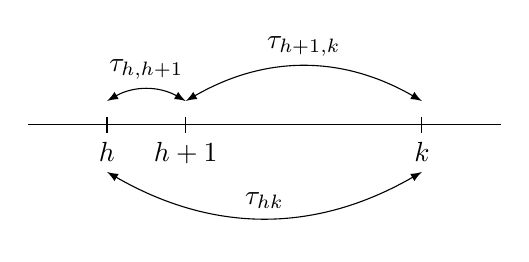
\begin{tikzpicture}
          % Line
          \draw[-] (-1,0) -- (5,0);
          % Integers
          \foreach \x/\label in {0/h, 1/h+1, 4/k} {
            \draw(\x,0.1) -- (\x,-0.1) node[below] {\(\label\)};
          }
          % Arcs above
          \draw[latex-latex, bend left=30] (0, 0.3) to node[midway, above] 
            {\(\tau_{h,h+1}\)} (1, 0.3);
          \draw[latex-latex, bend left=30] (1, 0.3) to node[midway, above]
            {\(\tau_{h+1,k}\)} (4, 0.3);
          % Arc below
          \draw[latex-latex, bend right=30] (0, -0.6) to node[midway, above]
            {\(\tau_{hk}\)} (4, -0.6);
        \end{tikzpicture}
    $$
    i.e.,
    $$
        \tau_{hk} = \tau_{h,h+1}\tau_{h+1,k}\tau_{h,h+1},
    $$
    and the conclusion follows by induction on $k-h$.
    \renewcommand{\qedsymbol}{\sc qed}
\end{proof}

Let $G=\gen{x_1,\dots,x_{n-1}\mid R}$, where $R$ stands for the relations listed above.

\paragraph{Claim 1:}$|G|\le n!$

By induction on $n$, the case $n=1$ is trivial. For $n>1$, let $G_{n-1}$ be like $G$ with $n-1$ replacing $n$. Similarly, let $R_{n-1}$ denote the relations for $n-1$. Hence,
$$
    G_{n-1}=\gen{x_1,\dots,x_{n-2}, R_{n-1}}
$$
By the inductive hypothesis we have $|G_{n-1}|\le (n-1)!$. Since $R_{n-1}\subseteq R$, we can use von Dyck's Theorem~\ref{von-dyck-thm} to conclude that there is an epimorphism $G\to G_{n-1}$. Hence, the claim will follow if we show that $|G:G_{n-1}|\le n$.

Since $\set{x_1,\dots,x_{n-1}}$ generates $G$, it is enough to verify that every $x_j$ permutes the $n$ right cosets
$$
    G_{n-1},\; G_{n-1}x_{n-1},\;\dots,\;G_{n-1}x_{n-1}\cdots x_1.
$$
For $1\le i\le n$ let $C_i$ denote the coset $G_{n-1}x_{n-1}\cdots x_i$. Note that $C_n=G_{n-1}$. There are five cases:
\begin{description}%[leftmargin=1.8cm,style=sameline]
    \item[$\underline{j<i-1}:$]
        \begin{align*}
            C_ix_j &= G_{n-1}x_{n-1}\cdots x_ix_j\\
                &= G_{n-1}x_jx_{n-1}\cdots x_i
                    &&;\ x_k\leftrightarrow x_j\\
                &= G_{n-1}x_{n-1}\cdots x_i
                    &&;\ x_j\in G_{n-1}\\
                &= C_i.
        \end{align*}
    \item[$\underline{j=i-1}:$] $C_ix_j=C_ix_{i-1}=C_{i-1}$.
    \item[$\underline{j=i}:$] Since $x_i^2=1$, $C_ix_j=C_ix_i=C_{i+1}$.
    \item[$\underline{j=i+1}:$]
        \begin{align*}
            C_ix_j &= C_ix_{i+1}\\
                &= C_{i+2}x_{i+1}x_ix_{i+1}\\
                &= C_{i+2}x_ix_{i+1}x_i
                    &&;\ (x_ix_{i+1})^3=1\\
                &= C_{i+2}x_{i+1}x_i
                    &&;\ i<(i+2)-1\\
                &= C_i.
        \end{align*}
    \item[$\underline{j>i+1}:$]
        \begin{align*}
            C_ix_j &= C_{j+1}x_jx_{j-1}x_{j-2}\cdots x_ix_j\\
                &= C_{j+1}x_jx_{j-1}x_jx_{j-2}\cdots x_i\\
                &= C_{j+1}x_{j-1}x_jx_{j-1}x_{j-2}\cdots x_i
                    &&;\ (x_{j-1}x_j)^3=1\\
                &= C_{j+1}x_jx_{j-1}x_{j-2}\cdots x_i
                    &&;\ j-1 < (j+1) -1\\
                &= C_i.
        \end{align*}
\end{description}

\paragraph{Claim 2:}$|G|\ge n!$

Let $\tau_{1,2},\dots,\tau_{n-1,n}$ be the $n-1$ adjacent permutations of $S_n$. Thus, the universal property of $G$ guaranties the existence of a commutative diagram
\begin{equation}\label{eq.G=S_n}
    \begin{tikzcd}
        {\set{x_1,\dots,x_{n-1}}}
                \arrow[d,"\tau"']
                \arrow[r,hook]
            &F
                \arrow[ld,"\tau^*"]
                \arrow[d,"\pi"]\\
        S_n
            &G
                \arrow[l,dashed,"\gamma"]
    \end{tikzcd}
\end{equation}
where $\tau(x_i)=\tau_{i,i+1}$. Given that, according to the lemma, $S=\gen{\im\tau}$, we deduce that $\tau^*$ is an epimorphism. Moreover, $\set{\tau_{12},\dots,\tau_{n-1,n}}$ satisfy the relations~$R$. Hence, by the von Dyck Theorem~\ref{von-dyck-thm}, the presentation $\pi$ induces an epimorphism $\gamma\colon G\to S_n$. In particular, $|G|\ge|S_n|=n!$.

\paragraph{Conclusion:} $\gamma:G\cong S_n$

This follows from the fact that $\im(\gamma)=S_n$, as shown by Claim~1 and Claim~2. Note also that, according to~$(\ref{eq.G=S_n})$, this isomorphism is the natural one that comes from the universal property of~$F$.

\end{proof}

\begin{xmpl}\label{example:group-of-order-21}
    Let $G$ be a nonabelian group or order $21$. Since $n_7(G)\mid3$ (Remark~\ref{p'-part}) and $n_7(G)\equiv 1\pmod 7$ (Corollary~\ref{p|n_p-1}), we deduce that there is only one subgroup $P$ of order $7$. Therefore $P\normal G$. If $Q\in\Syl_3(G)$, then $G=PQ$. Since $G$ is not abelian and both $P$ and $Q$ are cyclic, $n_3(G)>1$, otherwise $Q$ would be normal and consequently $P\leftrightarrow Q$. Since $n_3(G)\mid 7$, we deduce that $n_3(G)=7$.

    Given that $\Aut(\Z_7)$ is cyclic of order $7-1$, it contains $2$ elements of order~$3$, namely $\eta_2\colon x\mapsto 2x$ and $\eta_4\colon x\mapsto4x$, with $\eta_4=\eta_2^{-1}$. Therefore, there are two nontrivial morphisms from $\Z_3$ to $\Aut(\Z_7)$, one is $\phi_1\colon1\mapsto\eta_2$ and the other $\phi_2\colon 1\mapsto\eta_2^{-1}$.

    Consider the inversion $\tau\colon\Z_3\to\Z_3$ defined by $\tau(x)=-x$. Then $\phi_1\tau=\phi_2$ because
    $$
        \phi_1\tau(1)=\phi_1(-1)=\phi_1(1)^{-1}=\eta_2^{-1}(1)=\phi_2(1).
    $$
    Now define
    \begin{align*}
        \Phi\colon\Z_7\rtimes_{\phi_1}\Z_3&\to\Z_3\rtimes_{\phi_2}\Z_3\\
            (a,b)&\mapsto(a,\tau(b)).
    \end{align*}
    We have,
    \begin{align*}
        \Phi((a_1,b_1)\cdot_{\phi_1}(a_2,b_2))
            &= \Phi(a_1\phi_1(b_1)(a_2),b_1b_2)\\
            &= (a_1\phi_1(b_1)(a_2),\tau(b_1b_2))\\
            &= (a_1\phi_2(\tau(b_1))(a_2),\tau(b_1)\tau(b_2))
                &&;\ \tau^2=\id\\
            &= (a_1,\tau(b_1))\cdot_{\phi_2}(a_2,\tau(b_2))\\
            &= \Phi(a_1,b_1)\cdot_{\phi_2}\Phi(a_2,b_2),
    \end{align*}
    i.e., $\Phi$ is a morphism. Hence, an isomorphism. In conclusion, there is only one nonabelian group or order $21$, up to isomorphism [cf.~Lemma~\ref{semidirect-product-uniqueness}].

    Let now $B$ the group defined with generators and relations
    $$
        B = \gen{\sigma,\tau\mid \sigma^7=\tau^3=1,\,\sigma^2\tau=\tau\sigma}.
    $$
    Note that $\Z_7\rtimes\Z_3$ satisfies the same relations, for $\sigma=(1,0)$ and $\tau=(0,1)$. We can verify this using $\phi_1$ defined above,
    \begin{align*}
        \sigma^2\tau &= (1,0)(1,0)(0,1)\\
            &= (2,0)(0,1)\\
            &= (2,1)\\
        \tau\sigma &= (0,1)(1,0)\\
            &= (0+\eta_2(1),1)\\
            &= (2,1).
    \end{align*}
    By the von Dyck Theorem~\ref{von-dyck-thm}, there is an epimorphism $\pi\colon B\to\Z_7\times\Z_2$ that extends the map $\sigma\mapsto(1,0)$, $\tau\mapsto(0,1)$. Given that the products $\sigma^i\tau^j$ generate a subgroup that is normal in the free group, these products generate $B$. This implies that $\pi$ is a monomorphism because the exponents $i$ and $j$ are univocally determined in $\Z_7\rtimes\Z_3$.
\end{xmpl}

